\section{EXPERIMENTAL SETUP}

\begin{figure*}[t]
    \centering
    \resizebox{\textwidth}{!}{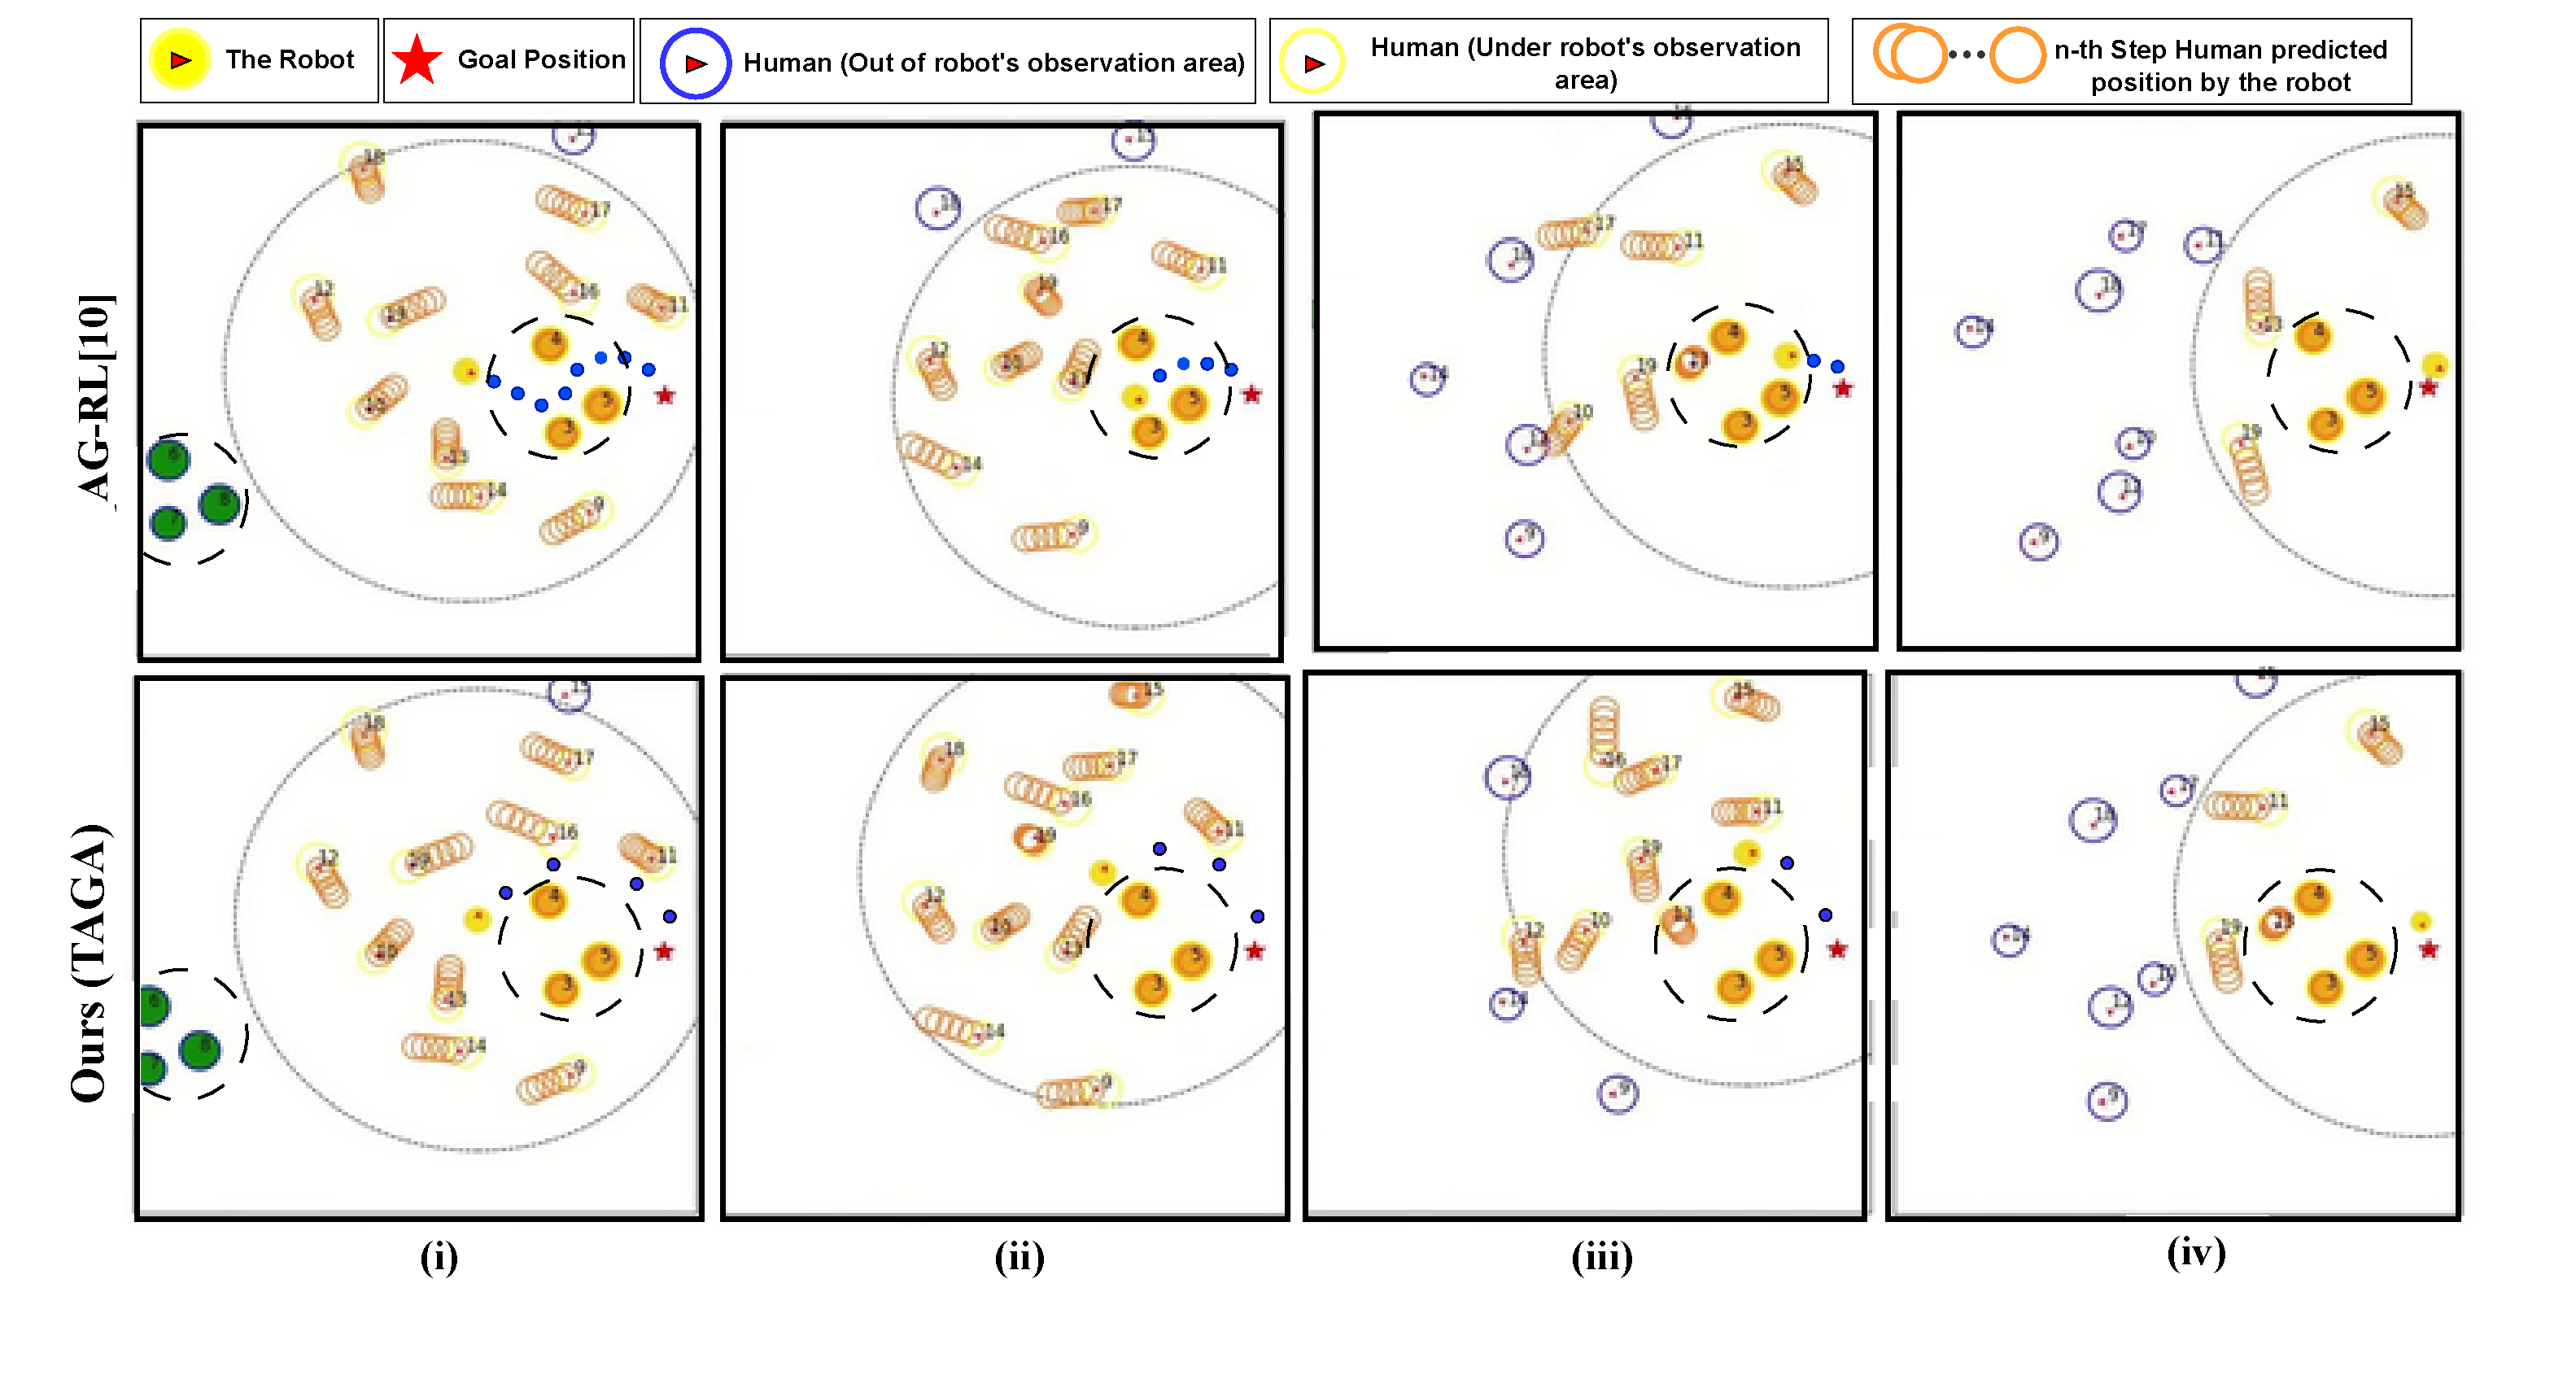
\includegraphics{figures/com.pdf}}
    \vspace{-25pt}
    \caption{\textbf{Comparison of our method (TAGA) and the state-of-the-art approach during the same testing episode, with identical randomized human and group placements.} The dotted circles represent group boundaries, while the small blue dots illustrate the robot's trajectory towards its goal. To ensure uninterrupted navigation, group collision constraints were disabled during the episode, allowing for continuous observation of the robot’s path planning and decision-making behavior.\UT{Try to address the 3rd review of reviwer 31289 and try to explain in qualilative sub section}
 }
    \vspace{-15pt}  
    \label{fig:sim-com}
\end{figure*}

\subsection{Simulation Environment}
We extend the crowd simulation framework from \cite{liu2023intention}, featuring a 12m × 12m space with up to 20 dynamic humans and a holonomic robot with 5m sensing range. Our key contribution is integrating realistic group behaviors alongside individual pedestrians. Groups are detected in real-time using DBSCAN clustering ($\epsilon = 1.5$m, minimum size = 2) rather than ground truth labels. \UT{addressing reviewer concerns about oversimplified detection.}

Dynamic groups follow leader-follower dynamics where a randomly selected leader navigates using ORCA while followers maintain cohesion through velocity adjustment: $v_i = v_{leader} + k(c - p_i)$, where $k$ is the cohesion factor and $c$ is the group centroid. Static groups remain stationary, representing conversational clusters.

\subsection{Evaluation Scenarios}
To ensure robust evaluation, we test across five diverse scenarios (100 episodes each):

\begin{itemize}
\item \textbf{Dense Groups} (20 episodes): 4 groups in 8m × 8m space, testing navigation through tight formations
\item \textbf{Mixed 50-50} (20 episodes): 8 individuals and 8 grouped humans, evaluating mixed crowd handling
\item \textbf{Dynamic Groups} (20 episodes): 3 moving groups with leader-follower dynamics
\item \textbf{Crossing Groups} (20 episodes): Groups traversing perpendicular to robot's path
\item \textbf{Groups Only} (20 episodes): All 18 humans in groups, no individuals
\end{itemize}

% This diverse set addresses the reviewer's requirement for "dense groups, mixed scenarios, and dynamic formations" while testing TAGA's adaptability.

\subsection{Metrics}
We evaluate using traditional navigation metrics and our proposed Group Collision Rate:

\textbf{Terminal States}: Success Rate (SR), Collision Rate (CR), and Timeout Rate (TR), where SR + CR + TR = 1.

% \textbf{Group Collision Rate (GCR)}: Measures the percentage of navigation time spent within group boundaries:
% \begin{equation}
% \text{GCR} = \frac{1}{T} \sum_{t=1}^{T} \mathbb{I}(d(r_t, c_j) < R_j) \times 100\%
% \end{equation}
% where $\mathbb{I}$ is the indicator function, $d(r_t, c_j)$ is robot distance to group $j$'s centroid, and $R_j$ is the group radius. Crucially, GCR operates independently of terminal states, providing continuous assessment throughout episodes.

\textbf{Group Collision Rate (GCR)}: Measures the percentage of navigation time during which the robot violates other groups' boundaries:
\begin{equation}
\text{GCR} = \frac{1}{T} \sum_{t=1}^{T} \mathbb{I}(d(r_t, c_j) < R_j) \times 100\%,
\end{equation}
where $T = t_{\text{episode}} \cdot f_{\text{ctrl}}$ is the total number of discrete control time steps, and the controller frequency is fixed at $f_{\text{ctrl}} = 10$~Hz throughout all experiments. $\mathbb{I}(\cdot)$ is the indicator function that returns $1$ if the robot is inside another group's region and $0$ otherwise, $d(r_t, c_j)$ denotes the Euclidean distance between the robot position at time step $t$ and group $j$'s centroid $c_j$, and $R_j$ is the group radius. Since GCR is evaluated at every control step, it provides a continuous assessment of group-aware behavior across the entire episode, independent of terminal success or failure. \UT{Try to address the 4th review of reviwer 31281}



\textbf{Efficiency}: Navigation Time (NT) and Path Length (PL) for successful episodes.

% \subsection{Implementation Details}
% We evaluate four baseline methods—ORCA \cite{orca}, Social Force \cite{helbing1995social}, DS-RNN \cite{liu2020decentralized}, and AG-RL \cite{liu2023intention} with and without TAGA integration. Key parameters include: safety margin $S = 0.5$m, critical distance $d_{critical} = 0.3$m, personal distance $d_{personal} = 0.5$m, and detection confidence threshold $\tau = 0.8$. All methods are tested on identical scenarios using fixed random seeds for reproducibility. The safety controller operates at 10Hz, ensuring real-time collision avoidance during group maneuvers.
\subsection{Implementation Details}
We evaluate four baseline methods—ORCA \cite{orca}, Social Force \cite{helbing1995social}, DS-RNN \cite{liu2020decentralized}, and AG-RL \cite{liu2023intention} with and without TAGA integration. Key parameters include: safety margin $S = 0.5$m, critical distance $d_{critical} = 0.3$m, personal distance $d_{personal} = 0.5$m. All methods are tested on identical scenarios using fixed random seeds for reproducibility. The safety controller operates at 10Hz, ensuring real-time collision avoidance during group maneuvers.

% \vspace{-4pt}
% \section{CROWD ROBOT NAVIGATION BENCHMARK}
% \vspace{-12pt}
% \begin{figure*}[t]
%     \centering
%     \resizebox{\textwidth}{!}{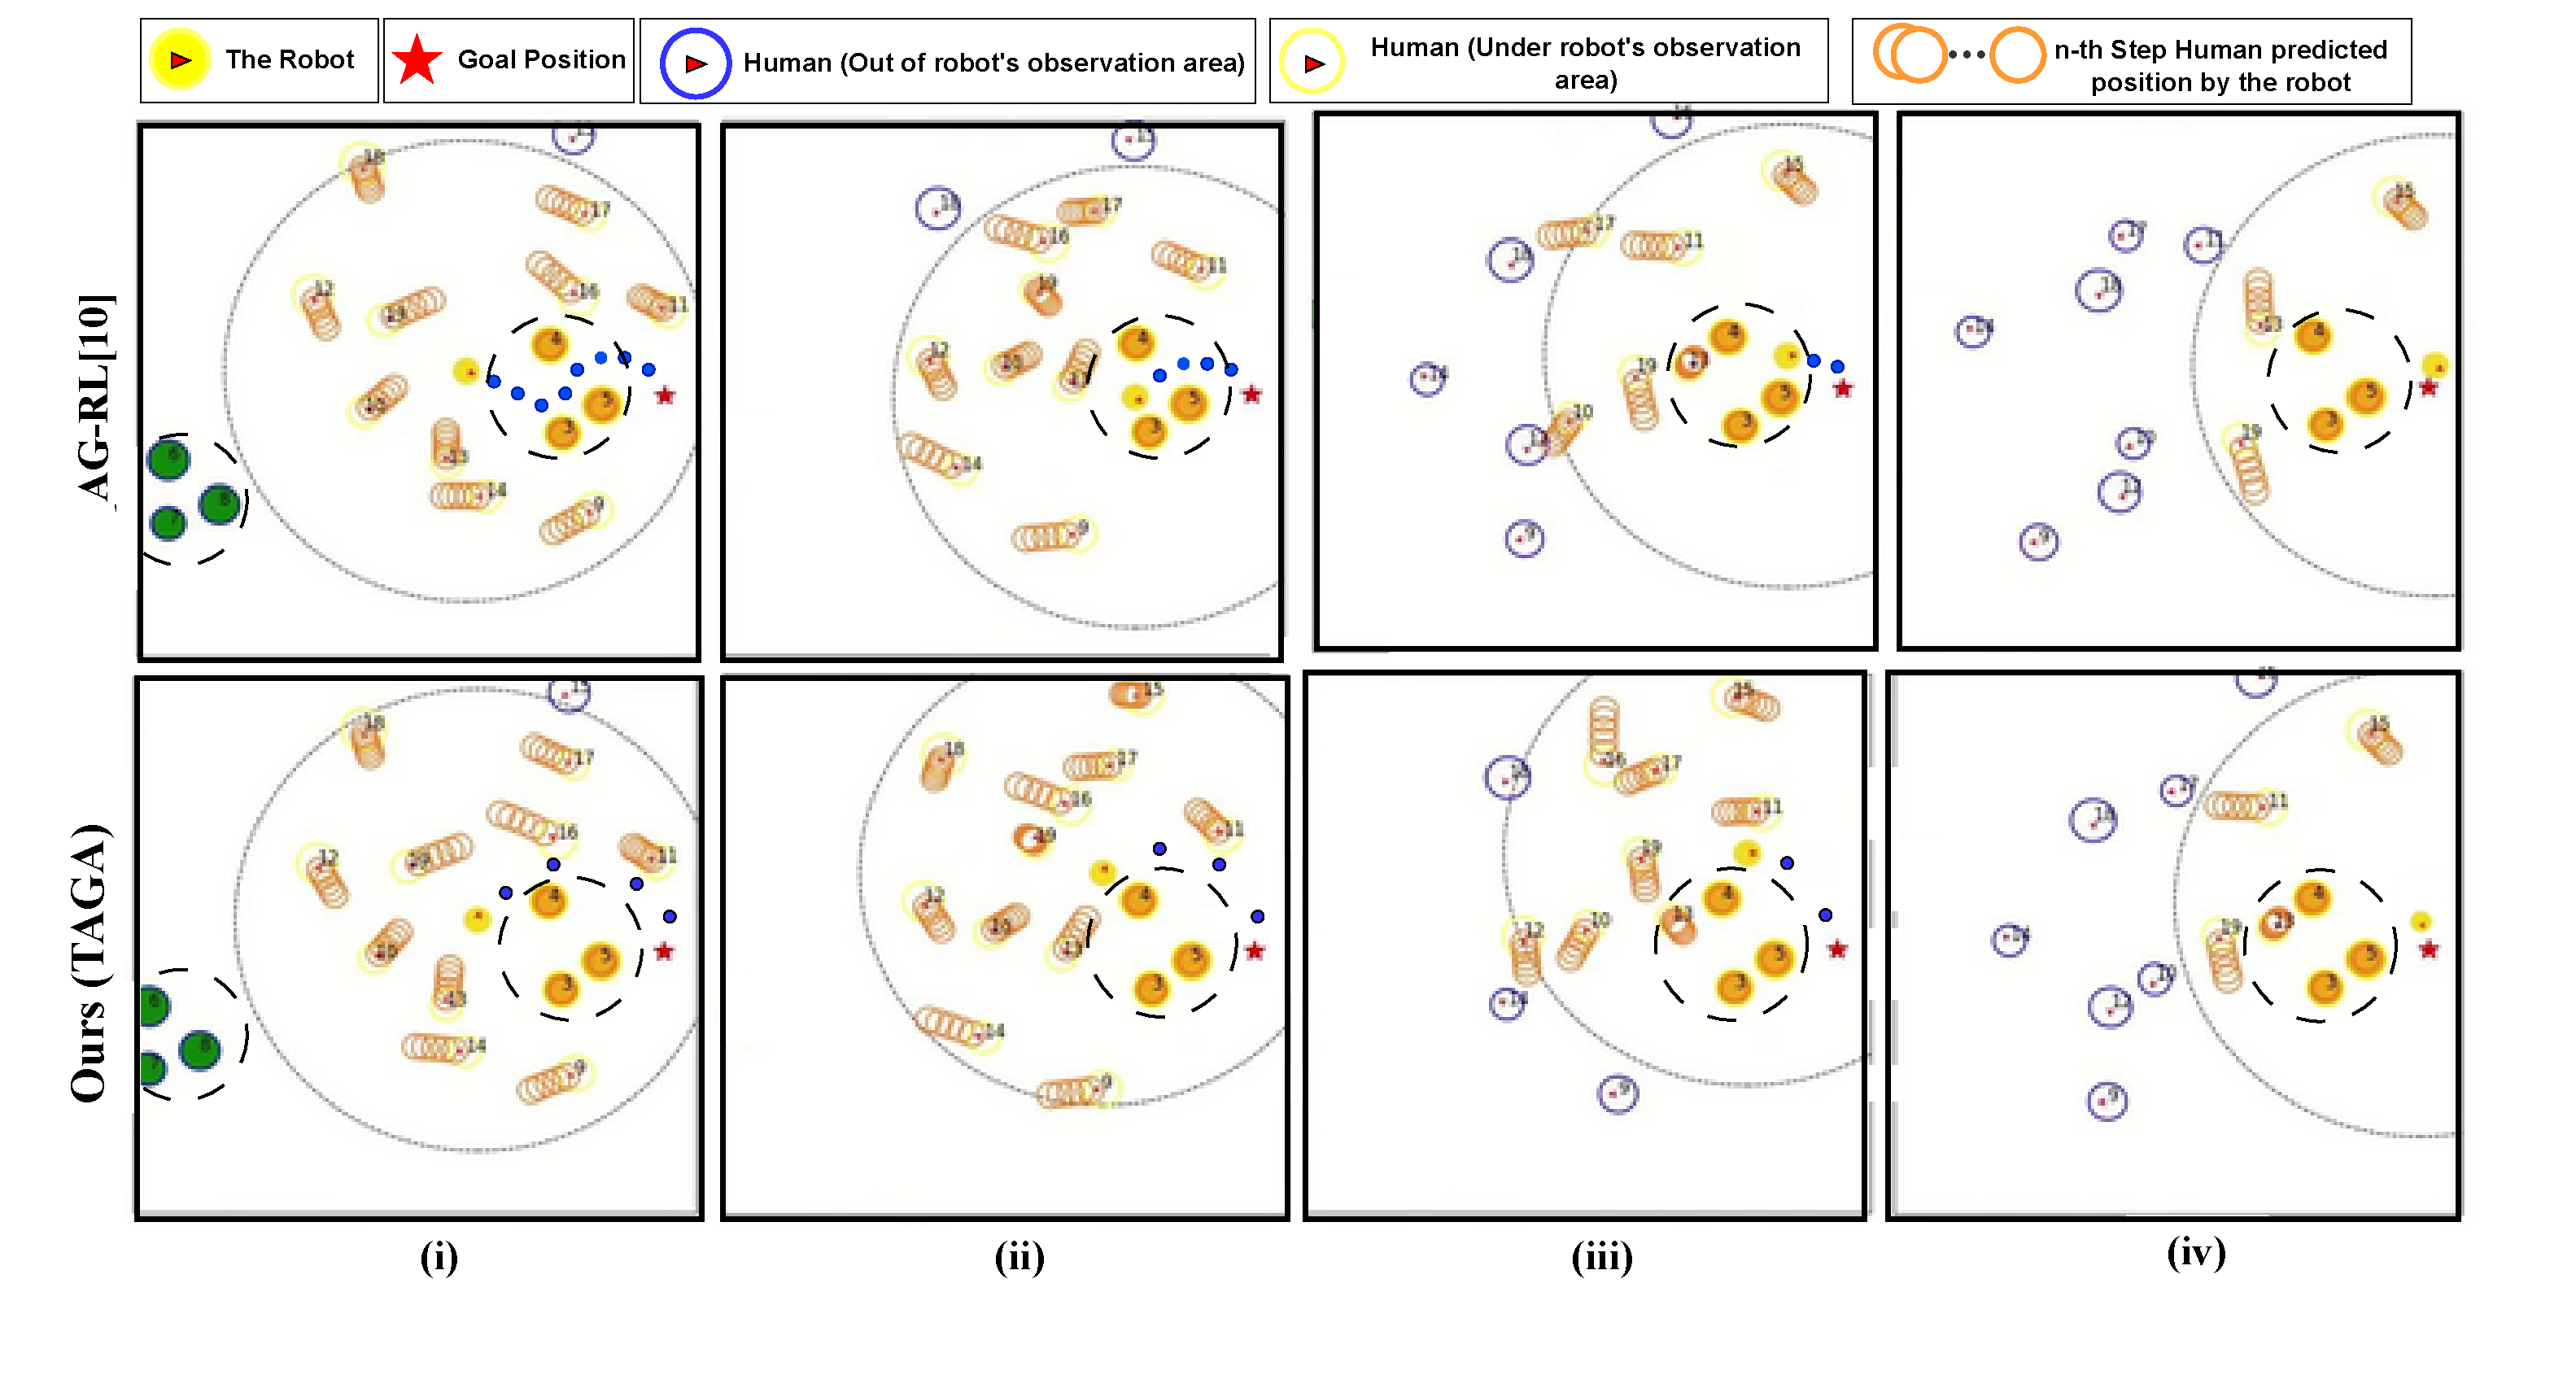
\includegraphics{figures/com.pdf}}
%     \vspace{-25pt}
%     \caption{\textbf{Comparison of our method (TAGA) and the state-of-the-art approach during the same testing episode, with identical randomized human and group placements.}  The dotted circles represent group boundaries, while the small blue dots illustrate the robot's trajectory towards its goal. To ensure uninterrupted navigation, group collision constraints were disabled during the episode, allowing for continuous observation of the robot’s path planning and decision-making behavior.
% }
%     \vspace{-15pt}  
%     \label{fig:sim-com}
% \end{figure*}

% \vspace{-2pt}
% \subsection{Simulation Environment}
% We build upon the simulation environment proposed in \cite{liu2023intention}, where a robot navigates through a dense 12m × 12m crowd space with up to 20 dynamic humans. The environment features a holonomic robot with a limited 5m sensor range and realistic human flow dynamics, ensuring continuous crowd interaction. Humans are controlled by the ORCA algorithm, reacting only to other humans while remaining unaware of the robot's presence.

% In contrast to \cite{liu2023intention}, we extend this environment by introducing human group behaviors alongside individual pedestrians. As shown in Fig. \ref{fig:sim-com}, groups are visually represented by similar-colored circles, indicating pedestrians that move together or standing close to each other. 
% This modification enables a more realistic evaluation of group-aware navigation strategies while preserving the original framework's crowd dynamics.
% \vspace{-10pt}
% \subsection{Human Group Simulation}
% We model human groups using a spatial representation, where each group is defined by a centroid $c$ and a radius $r$. The centroid $c$ is computed as the average position of all group members, where $N$ represents the total number of members in the group, and $p_i = (x_i, y_i)$ denotes the position of the $i$-th group member. Each group member is positioned within a maximum allowable distance $r$ from the centroid, ensuring spatial cohesion within the group. The set of all group members is represented by $G$:

% \begin{equation}
% c = \frac{1}{N} \sum_{i=1}^{N} p_i, \quad \| p_i - c \| \leq r, \quad \forall i \in G
% \end{equation}

% For dynamic groups, a leader is selected randomly from the group members:  

% \begin{equation}
% \text{leader} = \text{random}(G)
% \end{equation}

% We model human groups spatially, where each group is defined by a centroid $c$ and radius $r$. The centroid is the average position of all members, with $p_i = (x_i, y_i)$ representing the position of the $i$-th member. The members are constrained within a maximum distance $r$ from the centroid, ensuring spatial cohesion. The set of all members is denoted by $G$, and the spatial constraints are expressed as $c = \frac{1}{N} \sum_{i=1}^{N} p_i$, where $\quad \| p_i - c \| \leq r$ and $\quad \forall i \in G$.

% For dynamic groups, a leader is randomly selected as $\text{leader} = \text{random}(G)$.


% The leader follows ORCA-based navigation\cite{orca}, where $p_{\text{leader}}(t)$ represents the leader's position at time $t$, $v_{\text{orca}}$ is the velocity computed using the ORCA algorithm, and $\Delta t$ is the simulation time step:

% $$
% p_{\text{leader}}(t+1) = p_{\text{leader}}(t) + v_{\text{orca}} \cdot \Delta t \eqno{(3)}
% $$
% \vspace{-12pt} % Reduce space before

% \begin{equation}
% p_{\text{leader}}(t+1) = p_{\text{leader}}(t) + v_{\text{orca}} \cdot \Delta t
% \end{equation}
% \vspace{-14pt} % Reduce space before


% Each follower in the group maintains cohesion by adjusting its velocity relative to the leader and the group centroid. Here, $v_i$ denotes the velocity of the $i$-th follower, $v_{\text{leader}}$ represents the velocity of the leader, and $k$ is a cohesion factor ensuring that members remain within the group:

% $$
% v_i = v_{\text{leader}} + k (c - p_i) \eqno{(4)}
% $$
% \vspace{-10pt} % Reduce space before
% \begin{equation}
% v_i = v_{\text{leader}} + k (c - p_i)
% \end{equation}
% \vspace{-15pt} % Reduce space before

% For static groups, all members remain stationary, with $G_{\text{static}}$ representing the set of static group members, where $v_i = 0$ for all $i \in G_{\text{static}}$.

% This formulation ensures a structured simulation of both dynamic and static groups, allowing robots to interact with more realistic crowd behaviors in navigation environments.
% \vspace{-2pt}
% \subsection{Task}
% The robot, represented by a yellow circle with an arrow inside (Fig. \ref{fig:sim-com}), starts at one side of the environment, typically opposite to the goal, which is marked as a star in Fig. \ref{fig:sim-com}. The primary objective of the robot is to navigate toward the goal while avoiding collisions with individual humans, group members, and group boundaries. To prevent indefinite simulations in cases where a valid navigation path is not found, we impose a time limit of 197 steps. The robot navigates freely within the environment as the surrounding crowd, consisting of both individual pedestrians and group members, moves dynamically and unpredictably. However, humans in the crowd can traverse through group members without restrictions.

% \begin{figure}[!ht]
%     \centering
%     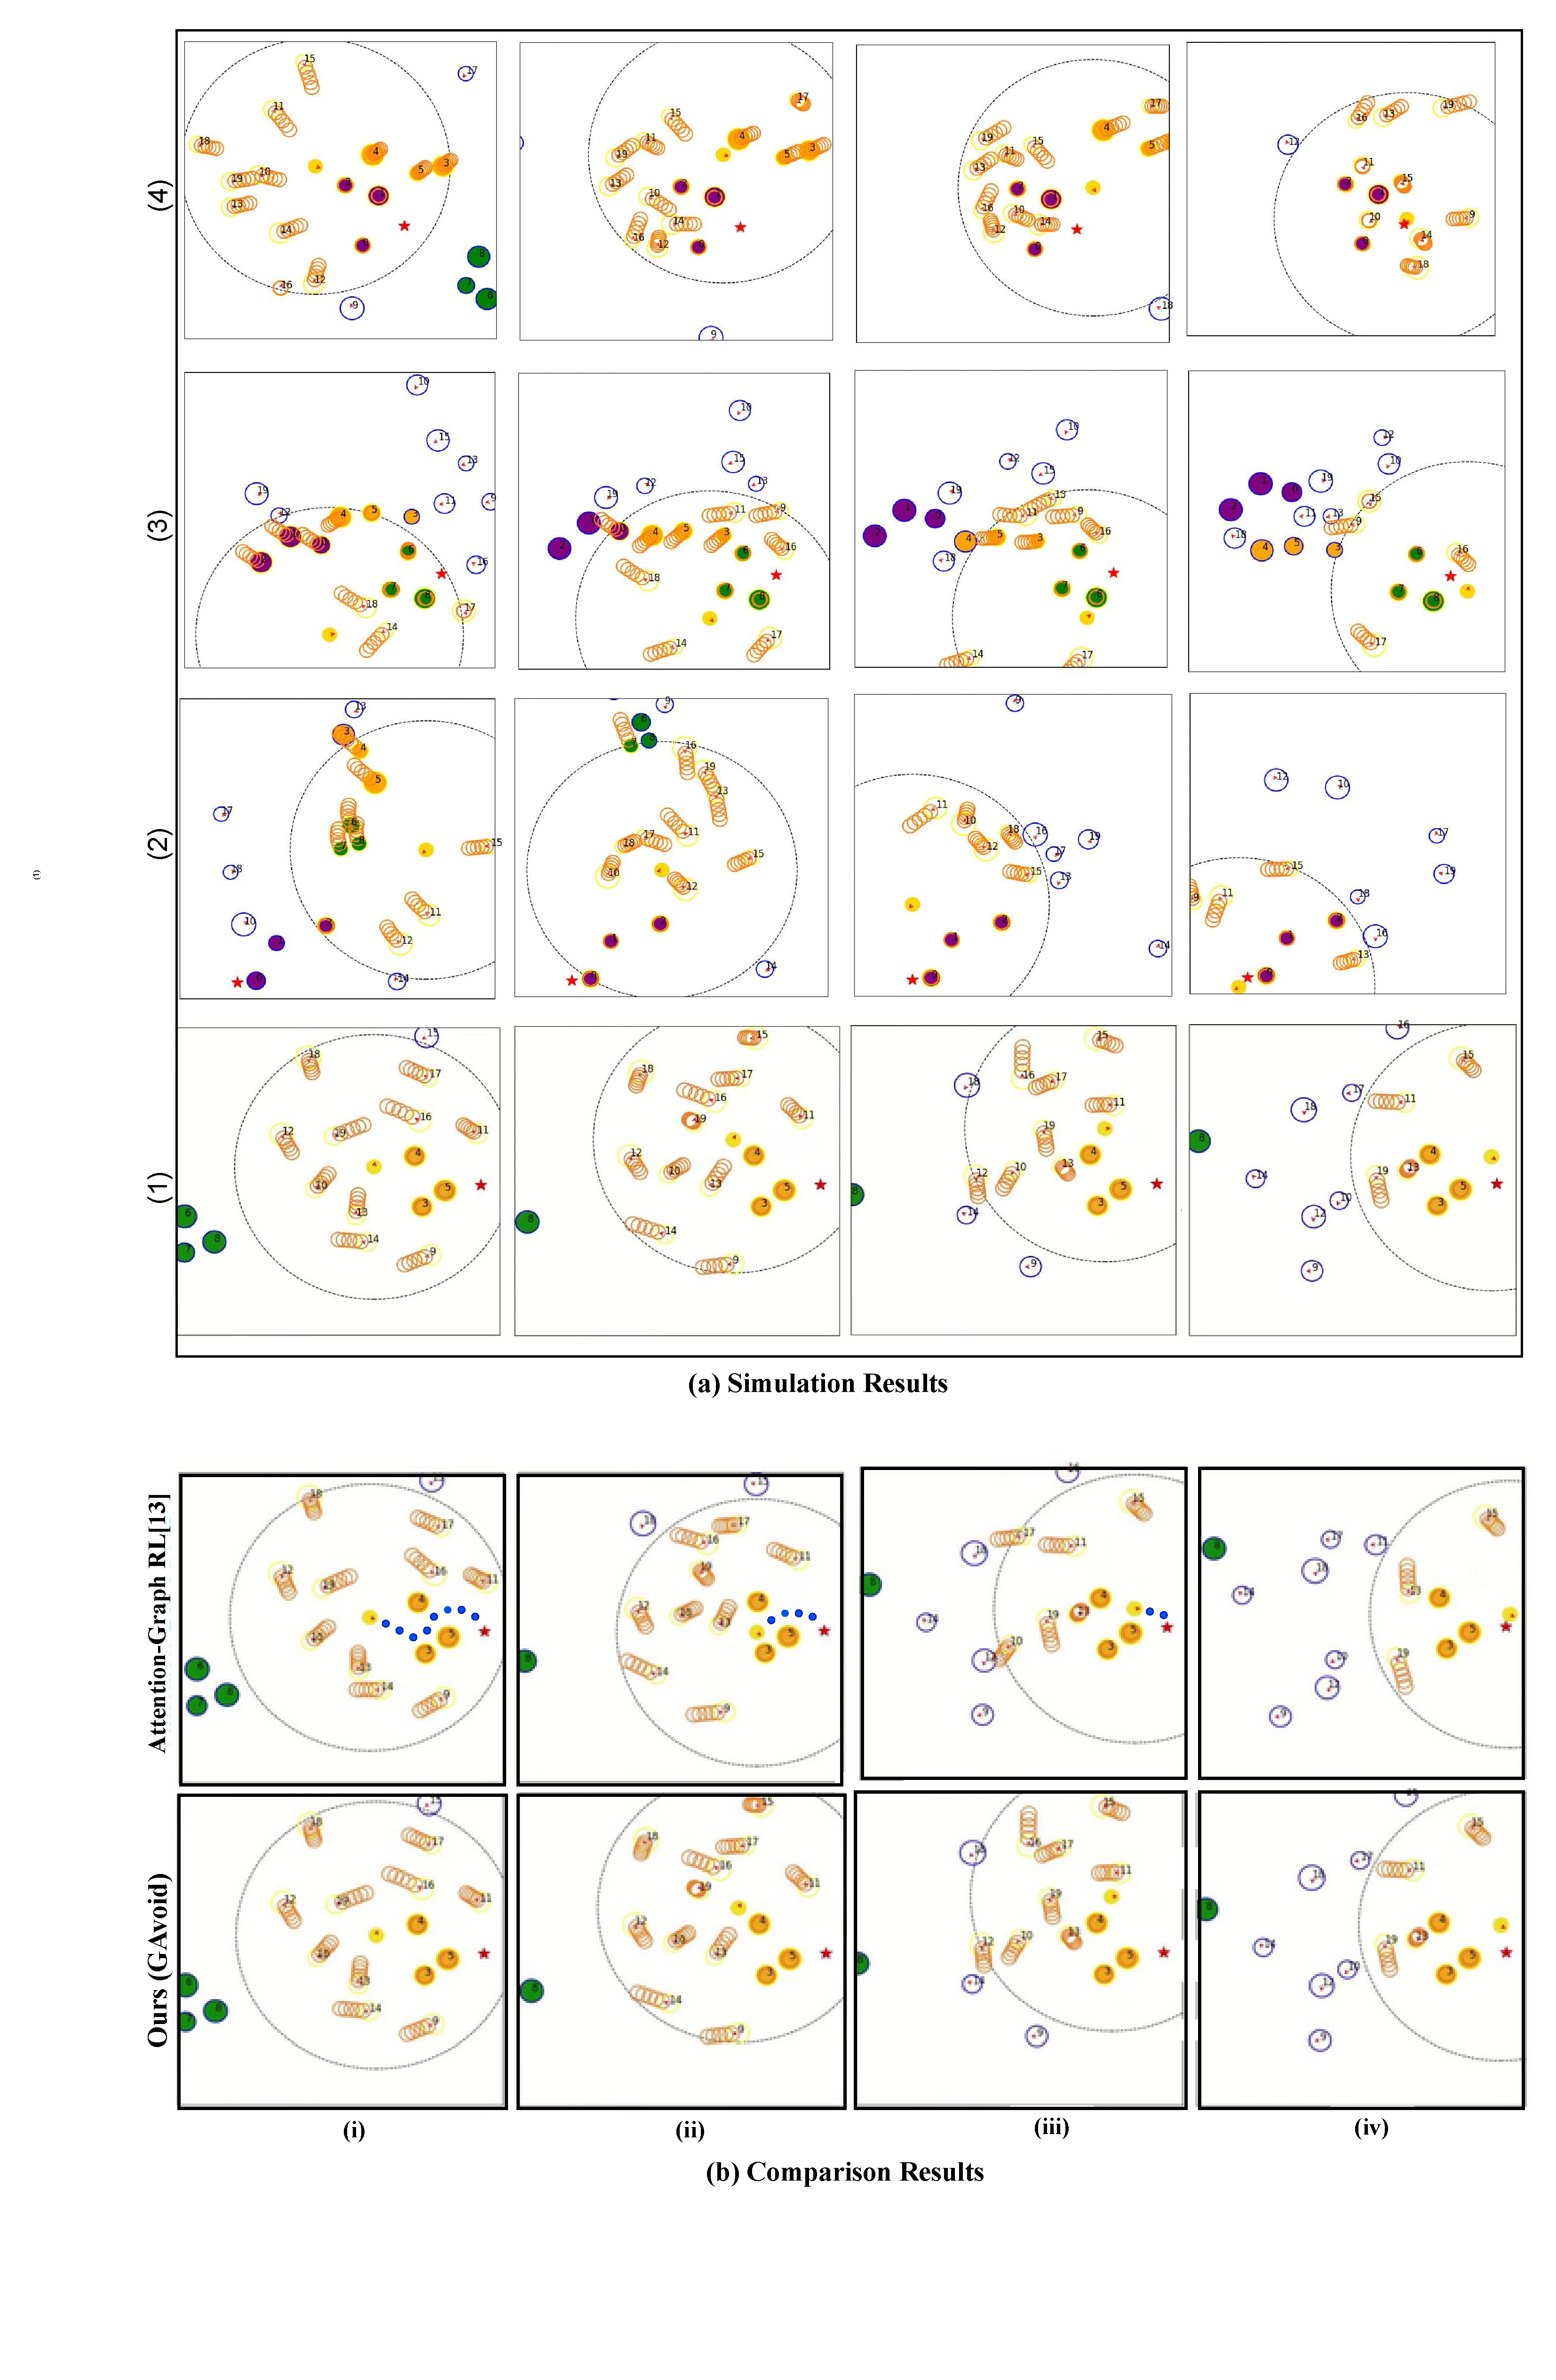
\includegraphics[width=0.5\textwidth]{figures/res.pdf}
%     \caption{Simulations Steps of different Configuration of Environments}
%     \label{fig:sim-res-1}
% \end{figure}
% \begin{figure}
%       \centering
%       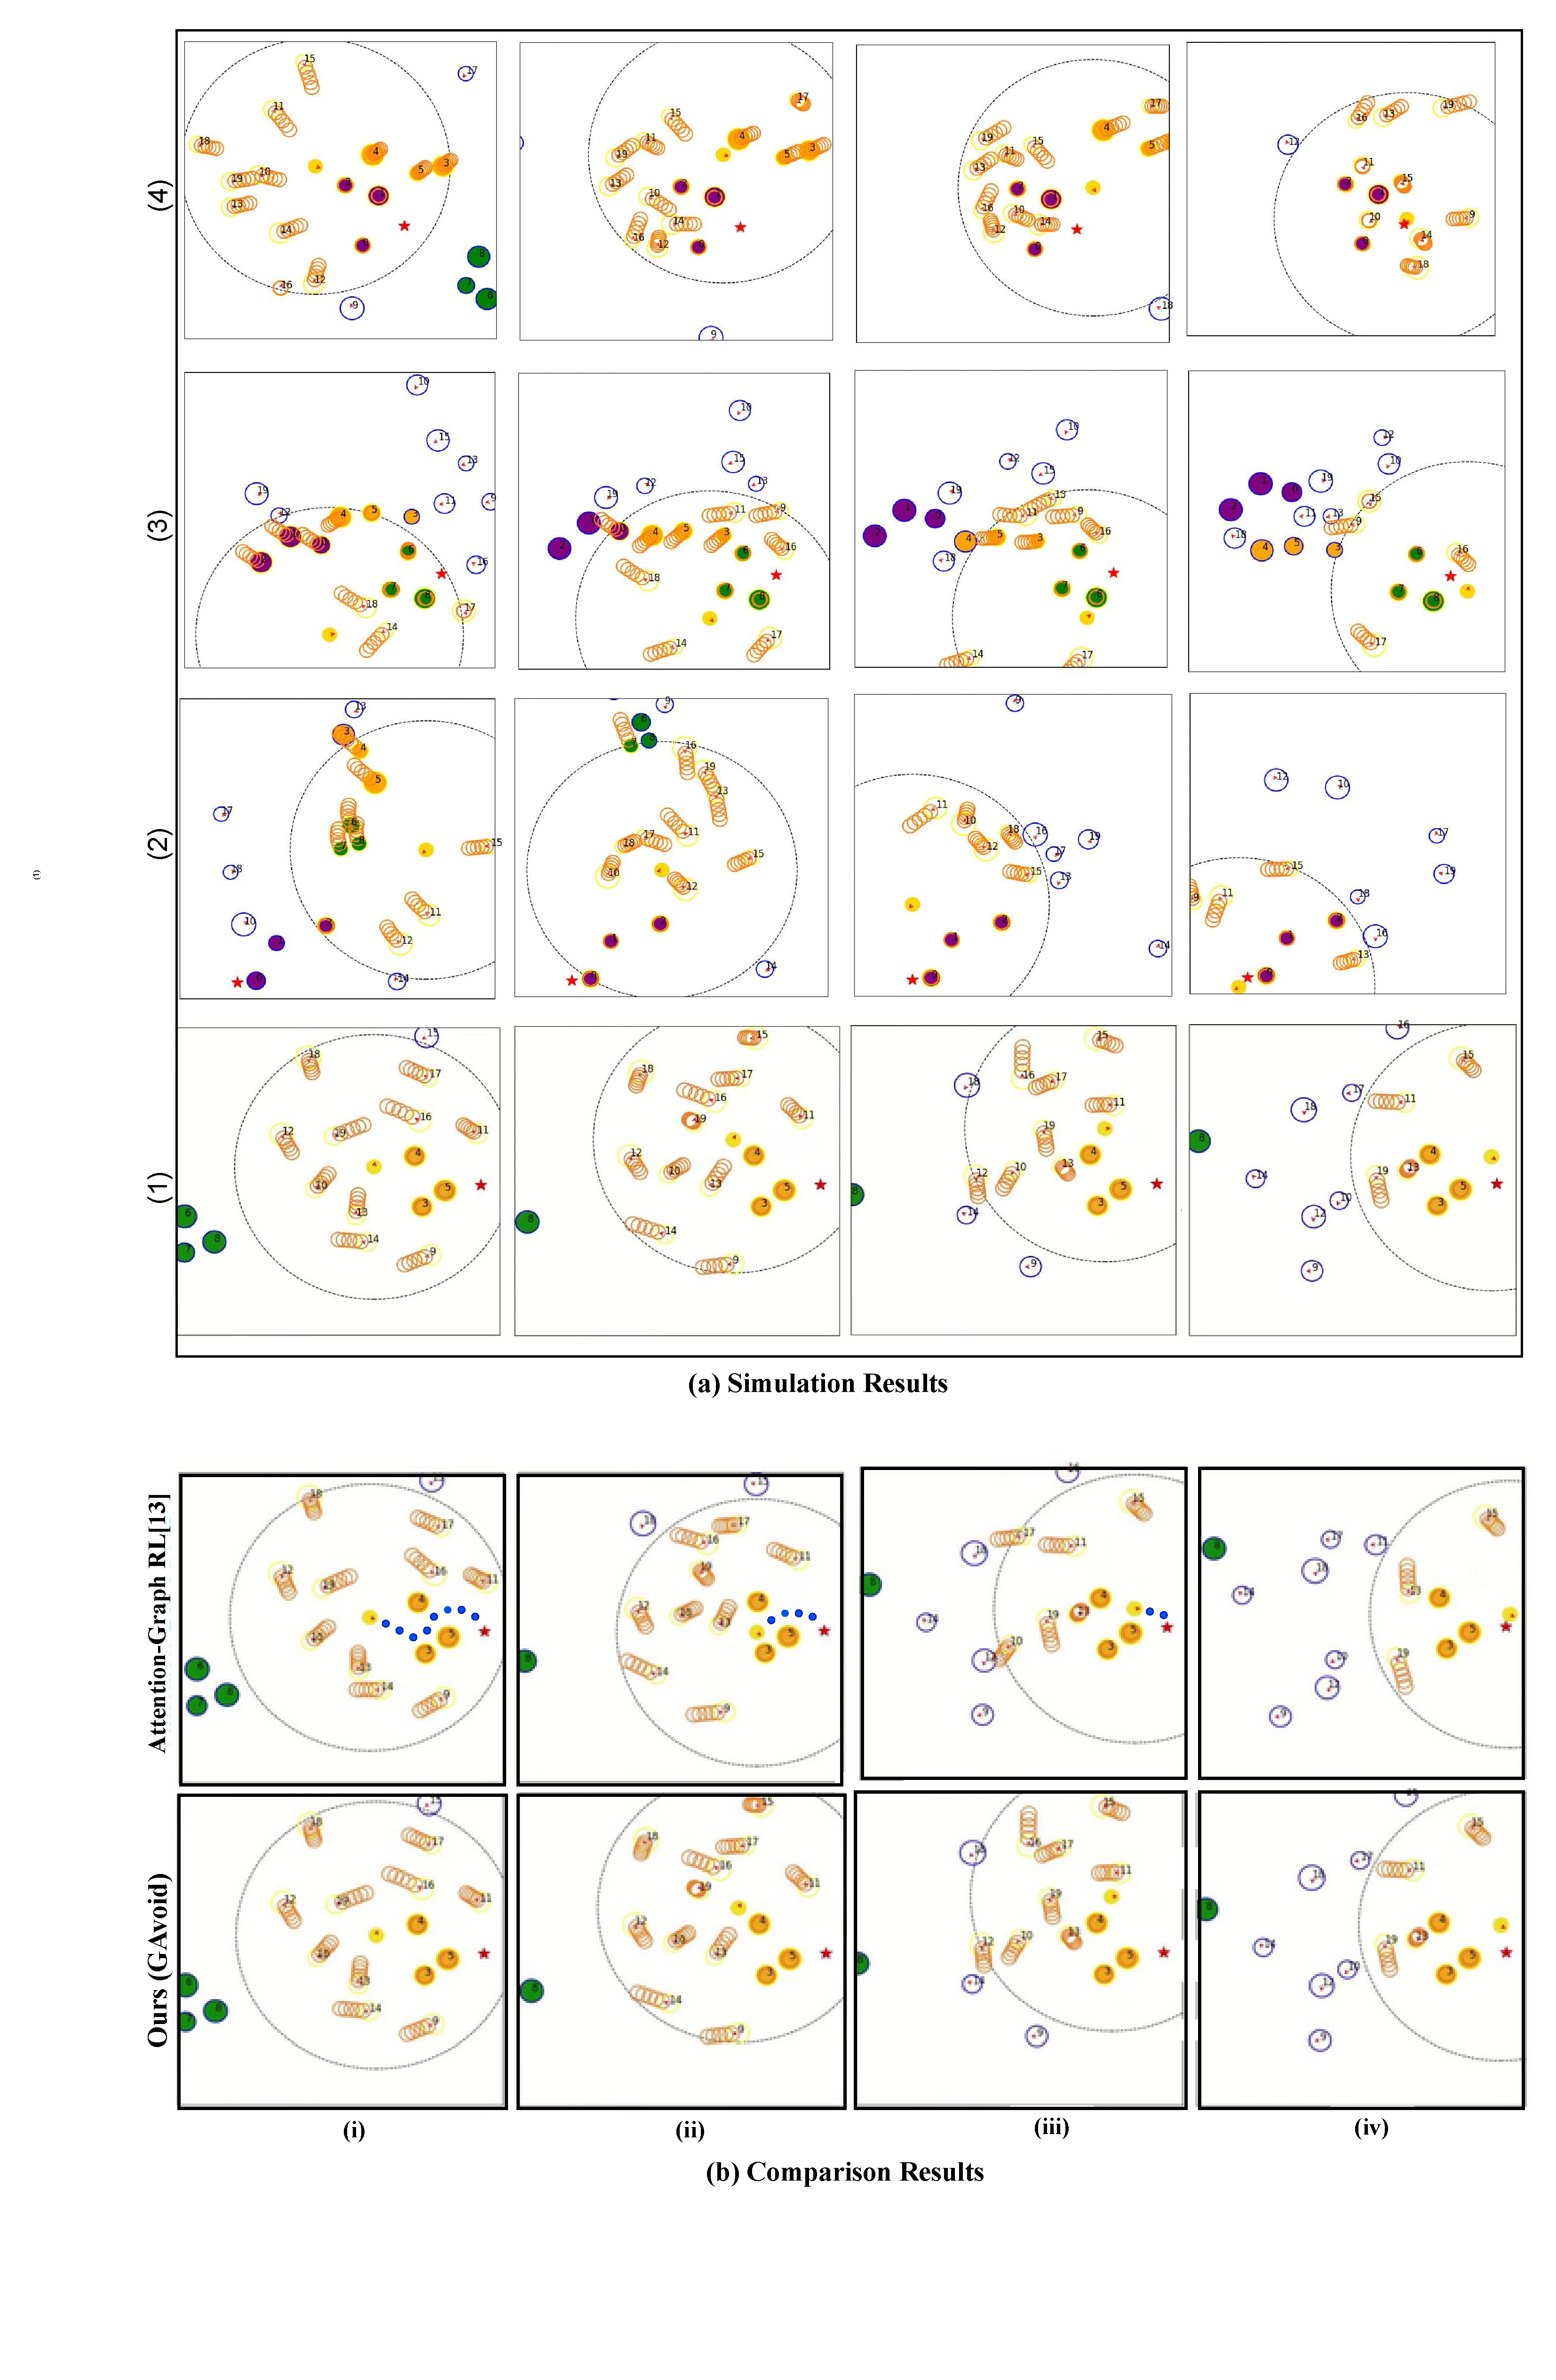
\includegraphics[scale=0.7]{figures/res.pdf}
%       \caption{Comparison with other models}
%       \label{fig:sim-com-1}
%    \end{figure}

% \vspace{-5pt}
% \vspace{-5pt} 
% \subsection{Benchmark Setup}
% To evaluate the impact of human groups on robot navigation, we conduct the benchmark in two experimental phases. First, we evaluate the performance of four widely used navigation frameworks—ORCA \cite{orca}, Social Force \cite{helbing1995social}, DS-RNN \cite{liu2020decentralized}, and AG-RL \cite{liu2023intention} to analyze their ability to navigate in the presence of individual humans and human groups. Next, we integrate our proposed TAGA mechanism into these models to examine how well they adapt to group-aware navigation. For instance, ORCA + TAGA allows ORCA to incorporate reactive group avoidance, ensuring that it respects group boundaries. Similar integration is applied to the other methods to assess their performance with group-awareness.

% Each approach is tested under identical conditions to ensure a fair comparison. The experiments are conducted across different configurations, adjusting crowd density, group sizes, and movement dynamics to assess performance across various scenarios.

% Furthermore, to quantify the effectiveness of group-aware navigation, GCR serves as a key performance metric, alongside traditional evaluation criteria such as SR, CR, and navigation efficiency. This benchmark setup provides a structured and reproducible evaluation of navigation models in realistic human environments.

% To ensure reliable evaluation, all methods are tested on 100 randomly generated unseen cases. If a collision occurs during an episode, the simulation is immediately terminated to reflect real-world navigation constraints. Consequently, the total of all failure rates, including Collision Rate (CR), Timeout Rate (TR), and GCR, along with the SR, always equals 1, expressed as $CR + TR + GCR + SR = 1$. Note that all time measurements are in seconds, and all distance measurements are in meters.
% \vspace{-5pt} 
% \subsection{Metrics}
% Our evaluation focuses on four key aspects: (1) robot navigation performance, (2) safety considerations, (3) real-time performance, and (4) group-aware navigation.

% \textbf{Real-Time Performance:} This metric evaluates the overall success of the navigation attempts, including the Success Rate (SR), which is the percentage of trials where the robot successfully reached the goal without colliding or exceeding the time limit.

% \textbf{Robot Navigation Performance:} These metrics assess the robot’s efficiency in reaching the goal while optimizing movement. This includes Navigation Time (NT), the average time required for the robot to reach the goal across all trials, and Path Length (PL), the total distance traveled by the robot from start to goal, averaged over all trials.

% \textbf{Safety Considerations:} These metrics quantify the safety of the robot’s navigation by measuring collision risks. They include CR, the number of trials where the robot collided with a human or group boundary, and TR, the percentage of trials where the robot failed to reach the goal within the allotted time.

% \textbf{Real-Time Performance:} This metric evaluates the overall success of the navigation attempts.

% \begin{itemize}
%     \item Success Rate (SR): The percentage of trials where the robot successfully reached the goal without colliding or exceeding the time limit.  
% \end{itemize}

% \textbf{Robot Navigation Performance:} These metrics assess the robot’s efficiency in reaching the goal while optimizing movement.

% \begin{itemize}
%     \item Navigation Time (NT): The average time required for the robot to reach the goal across all trials.  
%     \item Path Length (PL): The total distance traveled by the robot from start to goal, averaged over all trials.  
% \end{itemize}

% \textbf{Safety Considerations:} These metrics quantify the safety of the robot’s navigation by measuring collision risks.

% \begin{itemize}
%     \item Collision Rate (CR): The number of trials where the robot collided with a human or group boundary.  
%     \item Timeout Rate (TR): The percentage of trials where the robot failed to reach the goal within the allotted time.  
% \end{itemize}

% \textbf{Group-Aware Navigation:} To quantify the effectiveness of group-aware navigation, GCR measures how well the robot avoids intruding into human groups. Here, GCR is defined as the proportion of time the robot remains within a group’s spatial boundary during navigation:

% % $$
% % GCR = \frac{\sum_{t=1}^{T} \mathbb{I} (p_r(t) \in G)}{T} \eqno{(6)}
% % $$
% \vspace{-10pt}
% \begin{equation}
% GCR = \frac{\sum_{t=1}^{T} \mathbb{I} (p_r(t) \in G)}{T}
% \end{equation}
% \vspace{-15pt}

% where, $T$ is the total number of time steps in a trial, $p_r(t)$ represents the position of the robot at time step $t$, $\mathbb{I} (p_r(t) \in G)$ is an indicator function that returns 1 if the robot is inside a group's spatial boundary and 0 otherwise.


% We test all methods with 500 random unseen test cases. Our metrics include navigation metrics and social metrics. The navigation metrics measure the quality of the navigation and include the percentage success rate (SR), average navigation time (NT) in seconds, and path length (PL) in meters of the successful episodes. 



% \begin{figure}[t]
%       \centering
%       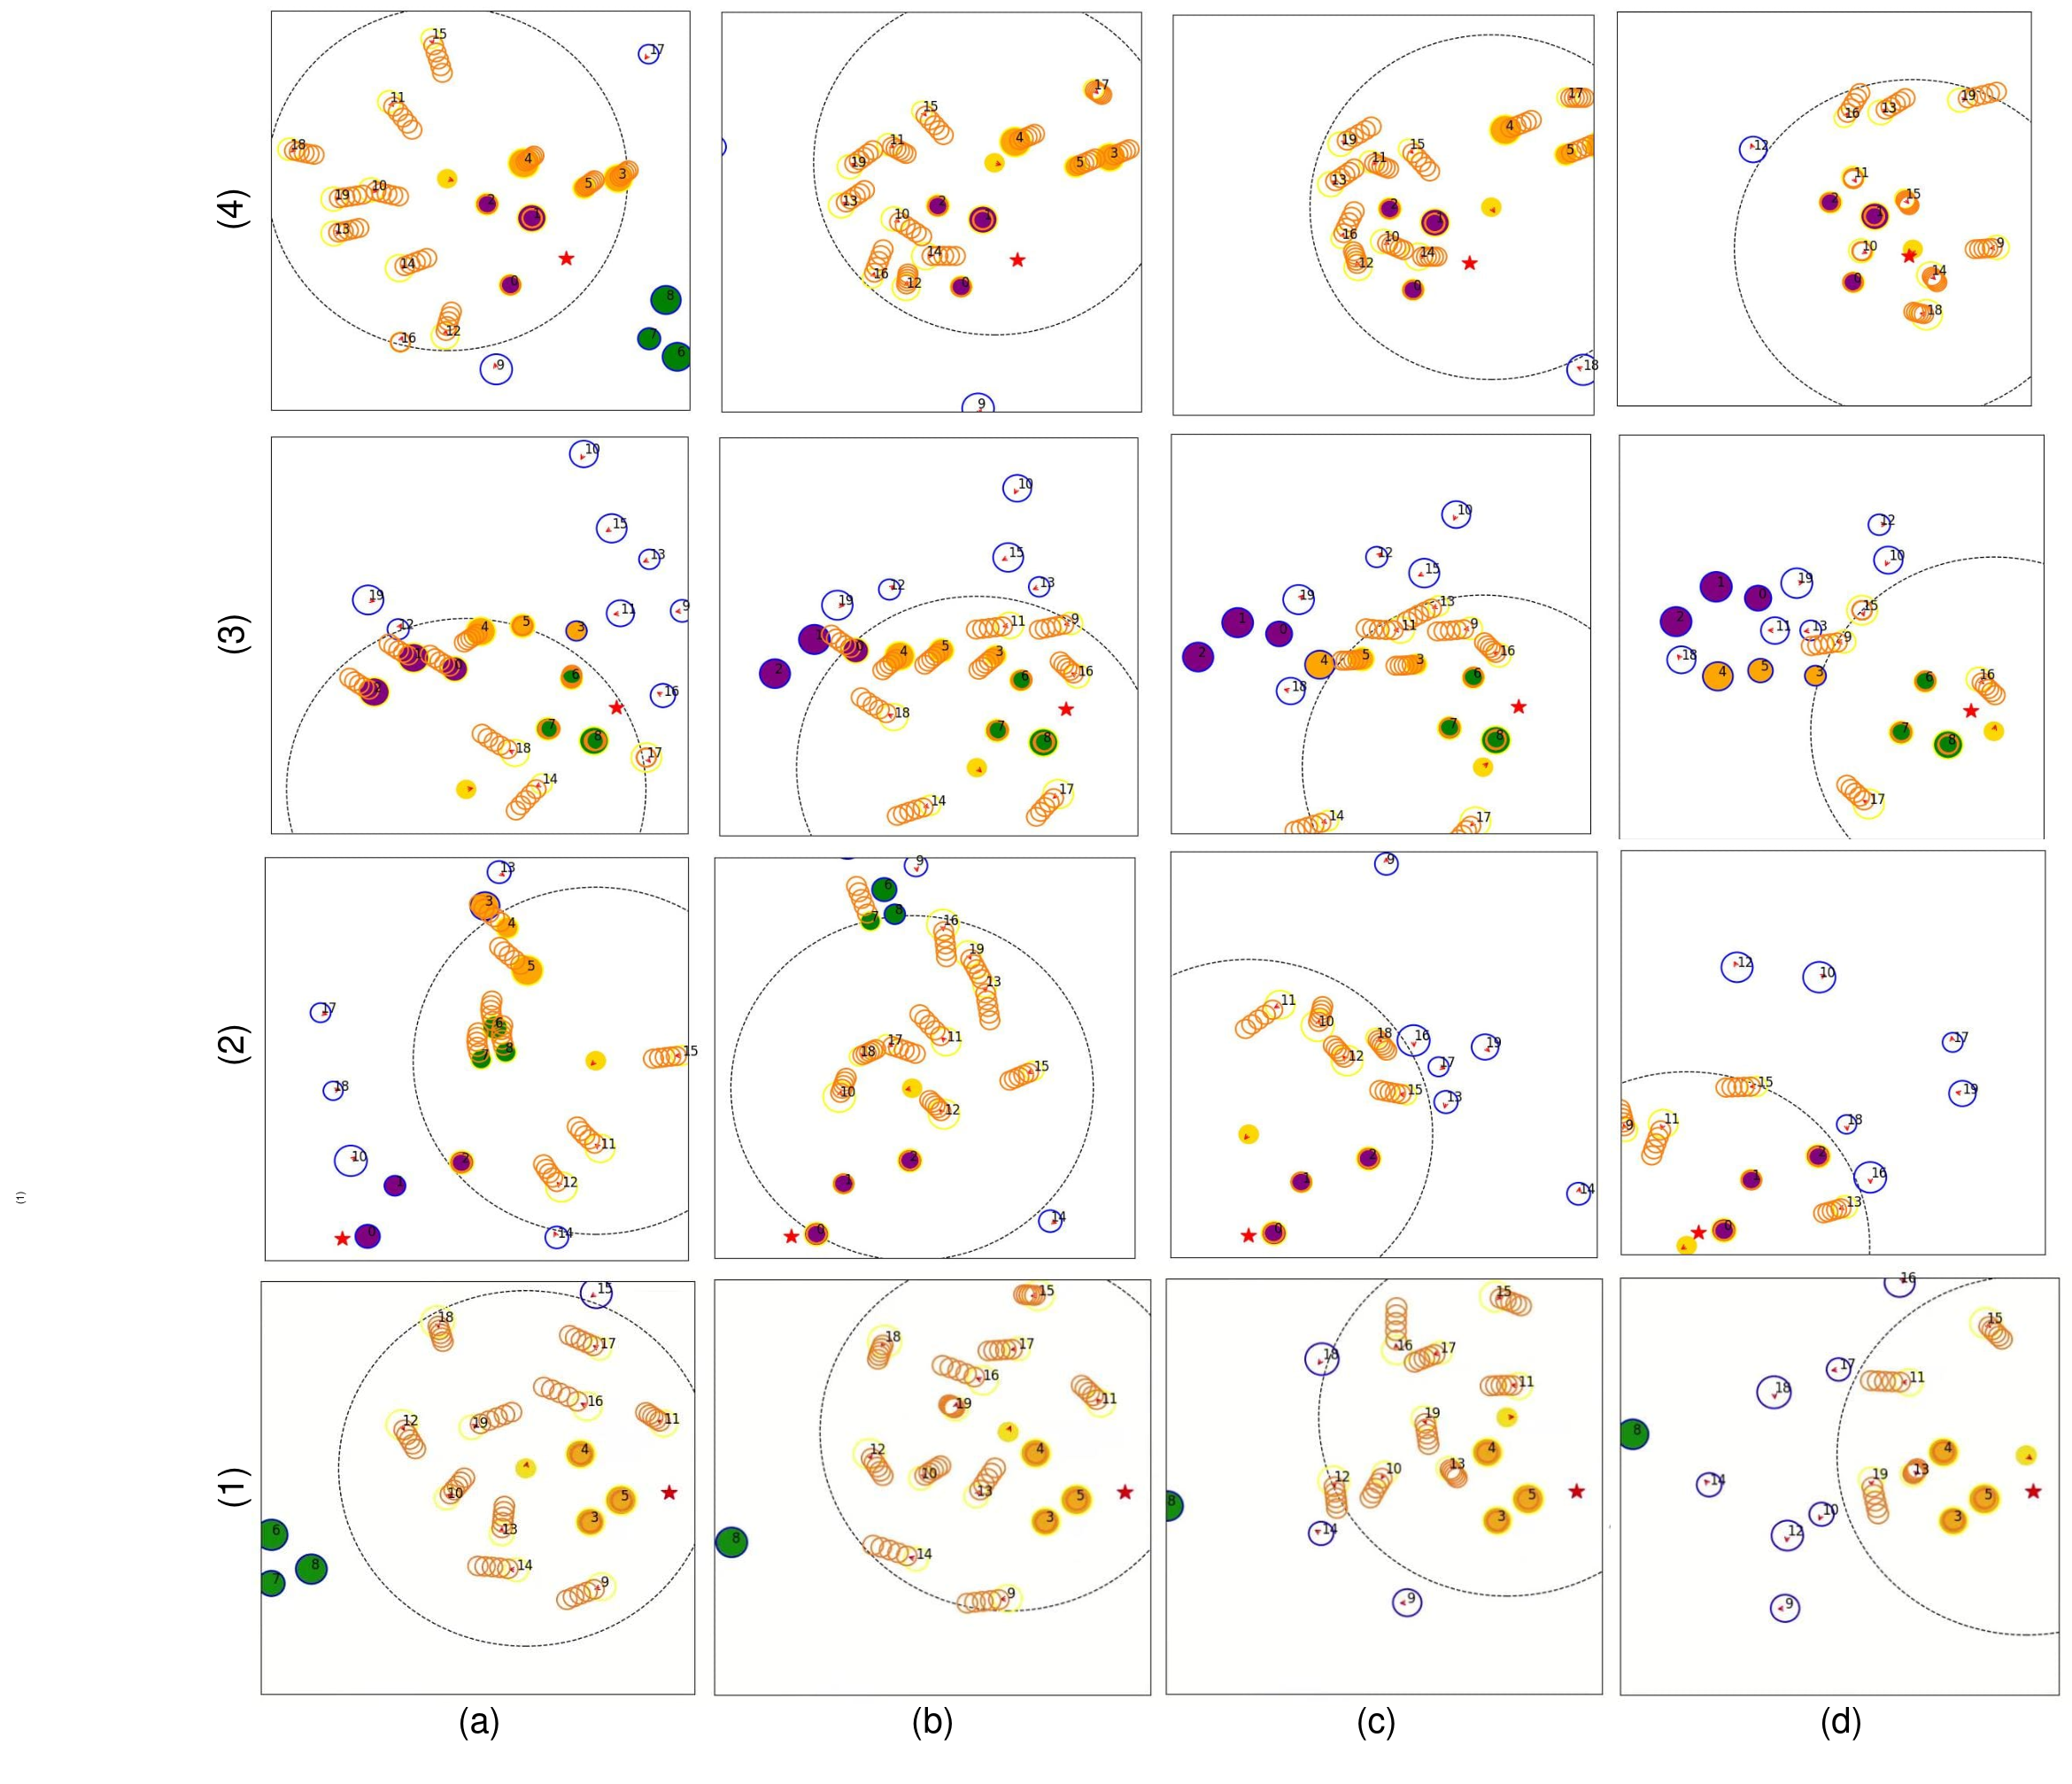
\includegraphics[scale=0.4]{figures/res-sim.png}
%       \caption{Simulations Steps of different Configuration of Environments}
%       \label{fig:sim-res-1}
%    \end{figure}























% \section{MATH}

% Before you begin to format your paper, first write and save the content as a separate text file. Keep your text and graphic files separate until after the text has been formatted and styled. Do not use hard tabs, and limit use of hard returns to only one return at the end of a paragraph. Do not add any kind of pagination anywhere in the paper. Do not number text heads-the template will do that for you.

% Finally, complete content and organizational editing before formatting. Please take note of the following items when proofreading spelling and grammar:

% \subsection{Abbreviations and Acronyms} Define abbreviations and acronyms the first time they are used in the text, even after they have been defined in the abstract. Abbreviations such as IEEE, SI, MKS, CGS, sc, dc, and rms do not have to be defined. Do not use abbreviations in the title or heads unless they are unavoidable.

% \subsection{Units}

% \begin{itemize}

% \item Use either SI (MKS) or CGS as primary units. (SI units are encouraged.) English units may be used as secondary units (in parentheses). An exception would be the use of English units as identifiers in trade, such as Ò3.5-inch disk driveÓ.
% \item Avoid combining SI and CGS units, such as current in amperes and magnetic field in oersteds. This often leads to confusion because equations do not balance dimensionally. If you must use mixed units, clearly state the units for each quantity that you use in an equation.
% \item Do not mix complete spellings and abbreviations of units: ÒWb/m2Ó or Òwebers per square meterÓ, not Òwebers/m2Ó.  Spell out units when they appear in text: Ò. . . a few henriesÓ, not Ò. . . a few HÓ.
% \item Use a zero before decimal points: Ò0.25Ó, not Ò.25Ó. Use Òcm3Ó, not ÒccÓ. (bullet list)

% \end{itemize}


% \subsection{Equations}

% The equations are an exception to the prescribed specifications of this template. You will need to determine whether or not your equation should be typed using either the Times New Roman or the Symbol font (please no other font). To create multileveled equations, it may be necessary to treat the equation as a graphic and insert it into the text after your paper is styled. Number equations consecutively. Equation numbers, within parentheses, are to position flush right, as in (1), using a right tab stop. To make your equations more compact, you may use the solidus ( / ), the exp function, or appropriate exponents. Italicize Roman symbols for quantities and variables, but not Greek symbols. Use a long dash rather than a hyphen for a minus sign. Punctuate equations with commas or periods when they are part of a sentence, as in

% $$
% \alpha + \beta = \chi \eqno{(1)}
% $$

% Note that the equation is centered using a center tab stop. Be sure that the symbols in your equation have been defined before or immediately following the equation. Use Ò(1)Ó, not ÒEq. (1)Ó or Òequation (1)Ó, except at the beginning of a sentence: ÒEquation (1) is . . .Ó

% \subsection{Some Common Mistakes}
% \begin{itemize}


% \item The word ÒdataÓ is plural, not singular.
% \item The subscript for the permeability of vacuum ?0, and other common scientific constants, is zero with subscript formatting, not a lowercase letter ÒoÓ.
% \item In American English, commas, semi-/colons, periods, question and exclamation marks are located within quotation marks only when a complete thought or name is cited, such as a title or full quotation. When quotation marks are used, instead of a bold or italic typeface, to highlight a word or phrase, punctuation should appear outside of the quotation marks. A parenthetical phrase or statement at the end of a sentence is punctuated outside of the closing parenthesis (like this). (A parenthetical sentence is punctuated within the parentheses.)
% \item A graph within a graph is an ÒinsetÓ, not an ÒinsertÓ. The word alternatively is preferred to the word ÒalternatelyÓ (unless you really mean something that alternates).
% \item Do not use the word ÒessentiallyÓ to mean ÒapproximatelyÓ or ÒeffectivelyÓ.
% \item In your paper title, if the words Òthat usesÓ can accurately replace the word ÒusingÓ, capitalize the ÒuÓ; if not, keep using lower-cased.
% \item Be aware of the different meanings of the homophones ÒaffectÓ and ÒeffectÓ, ÒcomplementÓ and ÒcomplimentÓ, ÒdiscreetÓ and ÒdiscreteÓ, ÒprincipalÓ and ÒprincipleÓ.
% \item Do not confuse ÒimplyÓ and ÒinferÓ.
% \item The prefix ÒnonÓ is not a word; it should be joined to the word it modifies, usually without a hyphen.
% \item There is no period after the ÒetÓ in the Latin abbreviation Òet al.Ó.
% \item The abbreviation Òi.e.Ó means Òthat isÓ, and the abbreviation Òe.g.Ó means Òfor exampleÓ.

% \end{itemize}

% % ########################
% % ########################
% % ########################
% \section{USING THE TEMPLATE}

% Use this sample document as your LaTeX source file to create your document. Save this file as {\bf root.tex}. You have to make sure to use the cls file that came with this distribution. If you use a different style file, you cannot expect to get required margins. Note also that when you are creating your out PDF file, the source file is only part of the equation. {\it Your \TeX\ $\rightarrow$ PDF filter determines the output file size. Even if you make all the specifications to output a letter file in the source - if your filter is set to produce A4, you will only get A4 output. }

% It is impossible to account for all possible situation, one would encounter using \TeX. If you are using multiple \TeX\ files you must make sure that the ``MAIN`` source file is called root.tex - this is particularly important if your conference is using PaperPlaza's built in \TeX\ to PDF conversion tool.

% \subsection{Headings, etc}

% Text heads organize the topics on a relational, hierarchical basis. For example, the paper title is the primary text head because all subsequent material relates and elaborates on this one topic. If there are two or more sub-topics, the next level head (uppercase Roman numerals) should be used and, conversely, if there are not at least two sub-topics, then no subheads should be introduced. Styles named ÒHeading 1Ó, ÒHeading 2Ó, ÒHeading 3Ó, and ÒHeading 4Ó are prescribed.

% \subsection{Figures and Tables}

% Positioning Figures and Tables: Place figures and tables at the top and bottom of columns. Avoid placing them in the middle of columns. Large figures and tables may span across both columns. Figure captions should be below the figures; table heads should appear above the tables. Insert figures and tables after they are cited in the text. Use the abbreviation ÒFig. 1Ó, even at the beginning of a sentence.

% \begin{table}[!t]
% \caption{An Example of a Table}
% \label{table_example}
% \begin{center}
% \begin{tabular}{|c||c|}
% \hline
% One & Two\\
% \hline
% Three & Four\\
% \hline
% \end{tabular}
% \end{center}
% \end{table}


%    \begin{figure}[thpb]
%       \centering
%       \framebox{\parbox{3in}{We suggest that you use a text box to insert a graphic (which is ideally a 300 dpi TIFF or EPS file, with all fonts embedded) because, in an document, this method is somewhat more stable than directly inserting a picture.
% }}
%       %\includegraphics[scale=1.0]{figurefile}
%       \caption{Inductance of oscillation winding on amorphous
%        magnetic core versus DC bias magnetic field}
%       \label{figurelabel}
%    \end{figure}
   

% Figure Labels: Use 8 point Times New Roman for Figure labels. Use words rather than symbols or abbreviations when writing Figure axis labels to avoid confusing the reader. As an example, write the quantity ÒMagnetizationÓ, or ÒMagnetization, MÓ, not just ÒMÓ. If including units in the label, present them within parentheses. Do not label axes only with units. In the example, write ÒMagnetization (A/m)Ó or ÒMagnetization {A[m(1)]}Ó, not just ÒA/mÓ. Do not label axes with a ratio of quantities and units. For example, write ÒTemperature (K)Ó, not ÒTemperature/K.Ó
